\documentclass[11pt]{article}

\usepackage[margin=1in]{geometry}
\usepackage{setspace}
\onehalfspacing
\usepackage{graphicx}
\graphicspath{report_images/}
\usepackage{appendix}
\usepackage{listings}
\usepackage{float}
\usepackage{multirow}
\usepackage{amsthm}
% The next three lines make the table and figure numbers also include section number
\usepackage{chngcntr}
\counterwithin{table}{section}
\counterwithin{figure}{section}
% Needed to make titling page without a page number
\usepackage{titling}

% DOCUMENT INFORMATION =================================================
\font\titleFont=cmr12 at 11pt
\title {{\titleFont ECEN 429: Introduction to Digital Systems Design Laboratory \\ North Carolina Agricultural and Technical State University \\ Department of Electrical and Computer Engineering}} % Declare Title
\author{\titleFont Reporter: Nikiyah Beulah \\ \titleFont Partner: Chris Cannon} % Declare authors
\date{\titleFont April 5, 2018}
% ======================================================================

\begin{document}

\begin{titlingpage}
\maketitle
\begin{center}
	Lab 10
\end{center}
\end{titlingpage}

\section{Introduction}
% Desc go here

\section{Background, Design Solution, and Results}

\subsection{Problem 1 }

\subsubsection{Background}
% Give background

\subsubsection{Design Solution}
% Describe Design

\begin{table}[H]
\begin{center}
\begin{tabular}{| l | l | l |}
	\hline
	Bit & Label & Port \\ \hline
	clk & Clock & W5 \\ \hline
	candy & Button Right & T17 \\ \hline
	gun & Button Left & W19 \\ \hline
	nickel & Button Top & T18 \\ \hline
	dime & Button Bottom & U17 \\ \hline
	reset & Button Center & U 18 \\ \hline
\end{tabular}
\caption{\label{tab:lab10_input_Ports}Input port assignments for  the vending machine.}
\end{center}
\end{table}

\begin{table}[H]
\begin{center}
\begin{tabular}{| l | l | l |}
	\hline
	Bit & Label & Port \\ \hline
	clk led & LED 15 & L1 \\ \hline
	amount 4 & LED 4 & W18 \\ \hline
	amount 3 & LED 3 & V19 \\ \hline
	amount 2 & LED 2 & U19 \\ \hline
	amount 1 & LED 1 & E19 \\ \hline
	amount 0 & LED 0 & U16 \\ \hline
\end{tabular}
\caption{\label{tab:lab10_output_Ports}Output port assignments for the vending machine.}
\end{center}
\end{table}

\begin{figure}
\begin{center}
	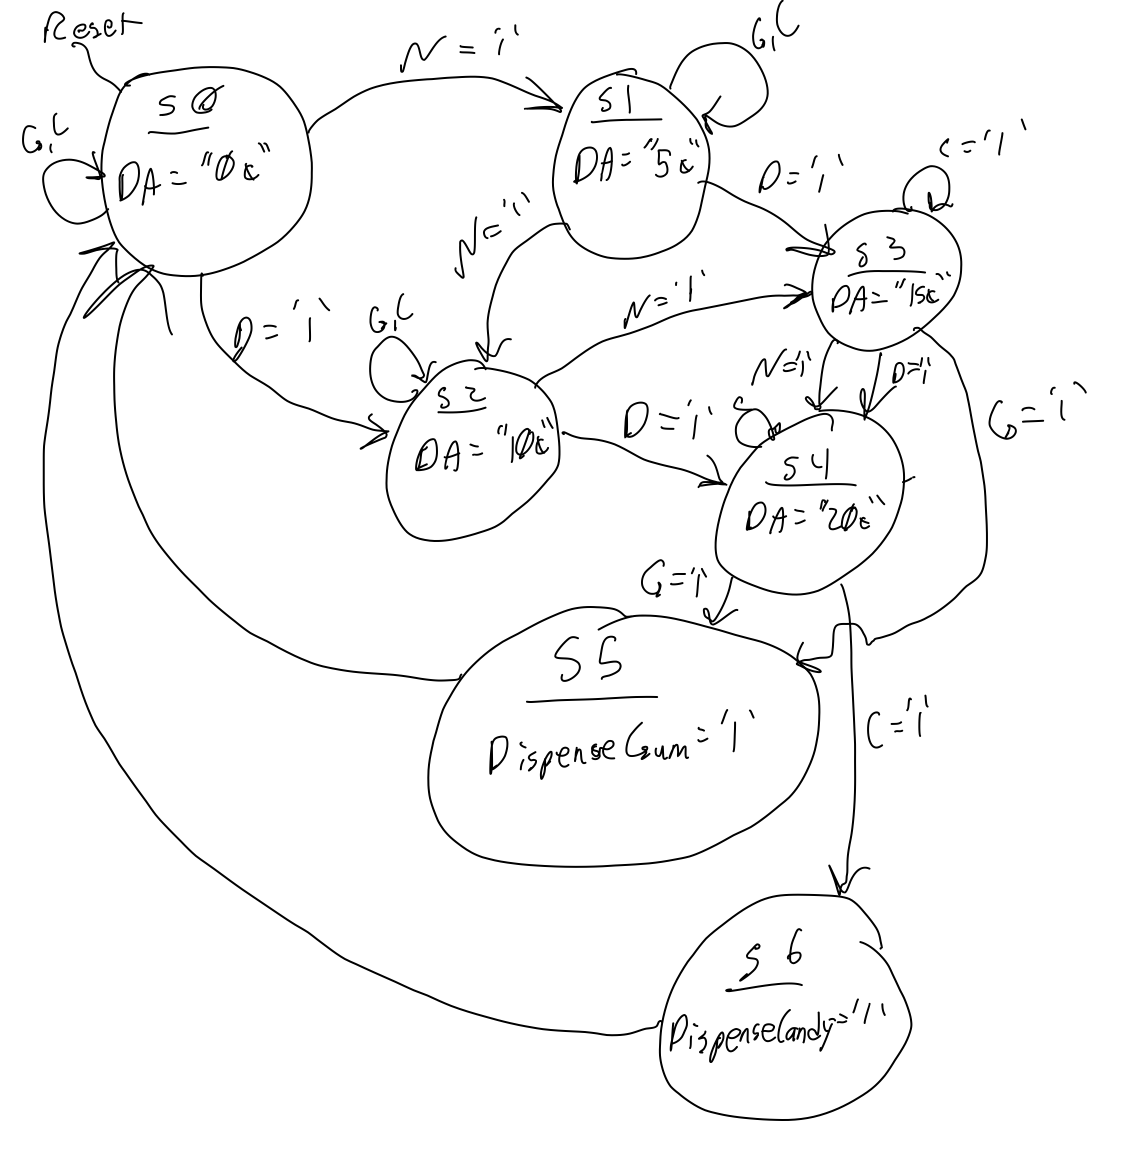
\includegraphics[width=0.5\textwidth]{./images/vendingMachineStateDiagram.png}
	\caption{\label{fig:lab10_state_diagram}State diagram for the vending machine implemented in this lab.}
\end{center}
\end{figure}

\subsubsection{Results}
% Describe Results

\begin{figure}[H]
\begin{center}
	%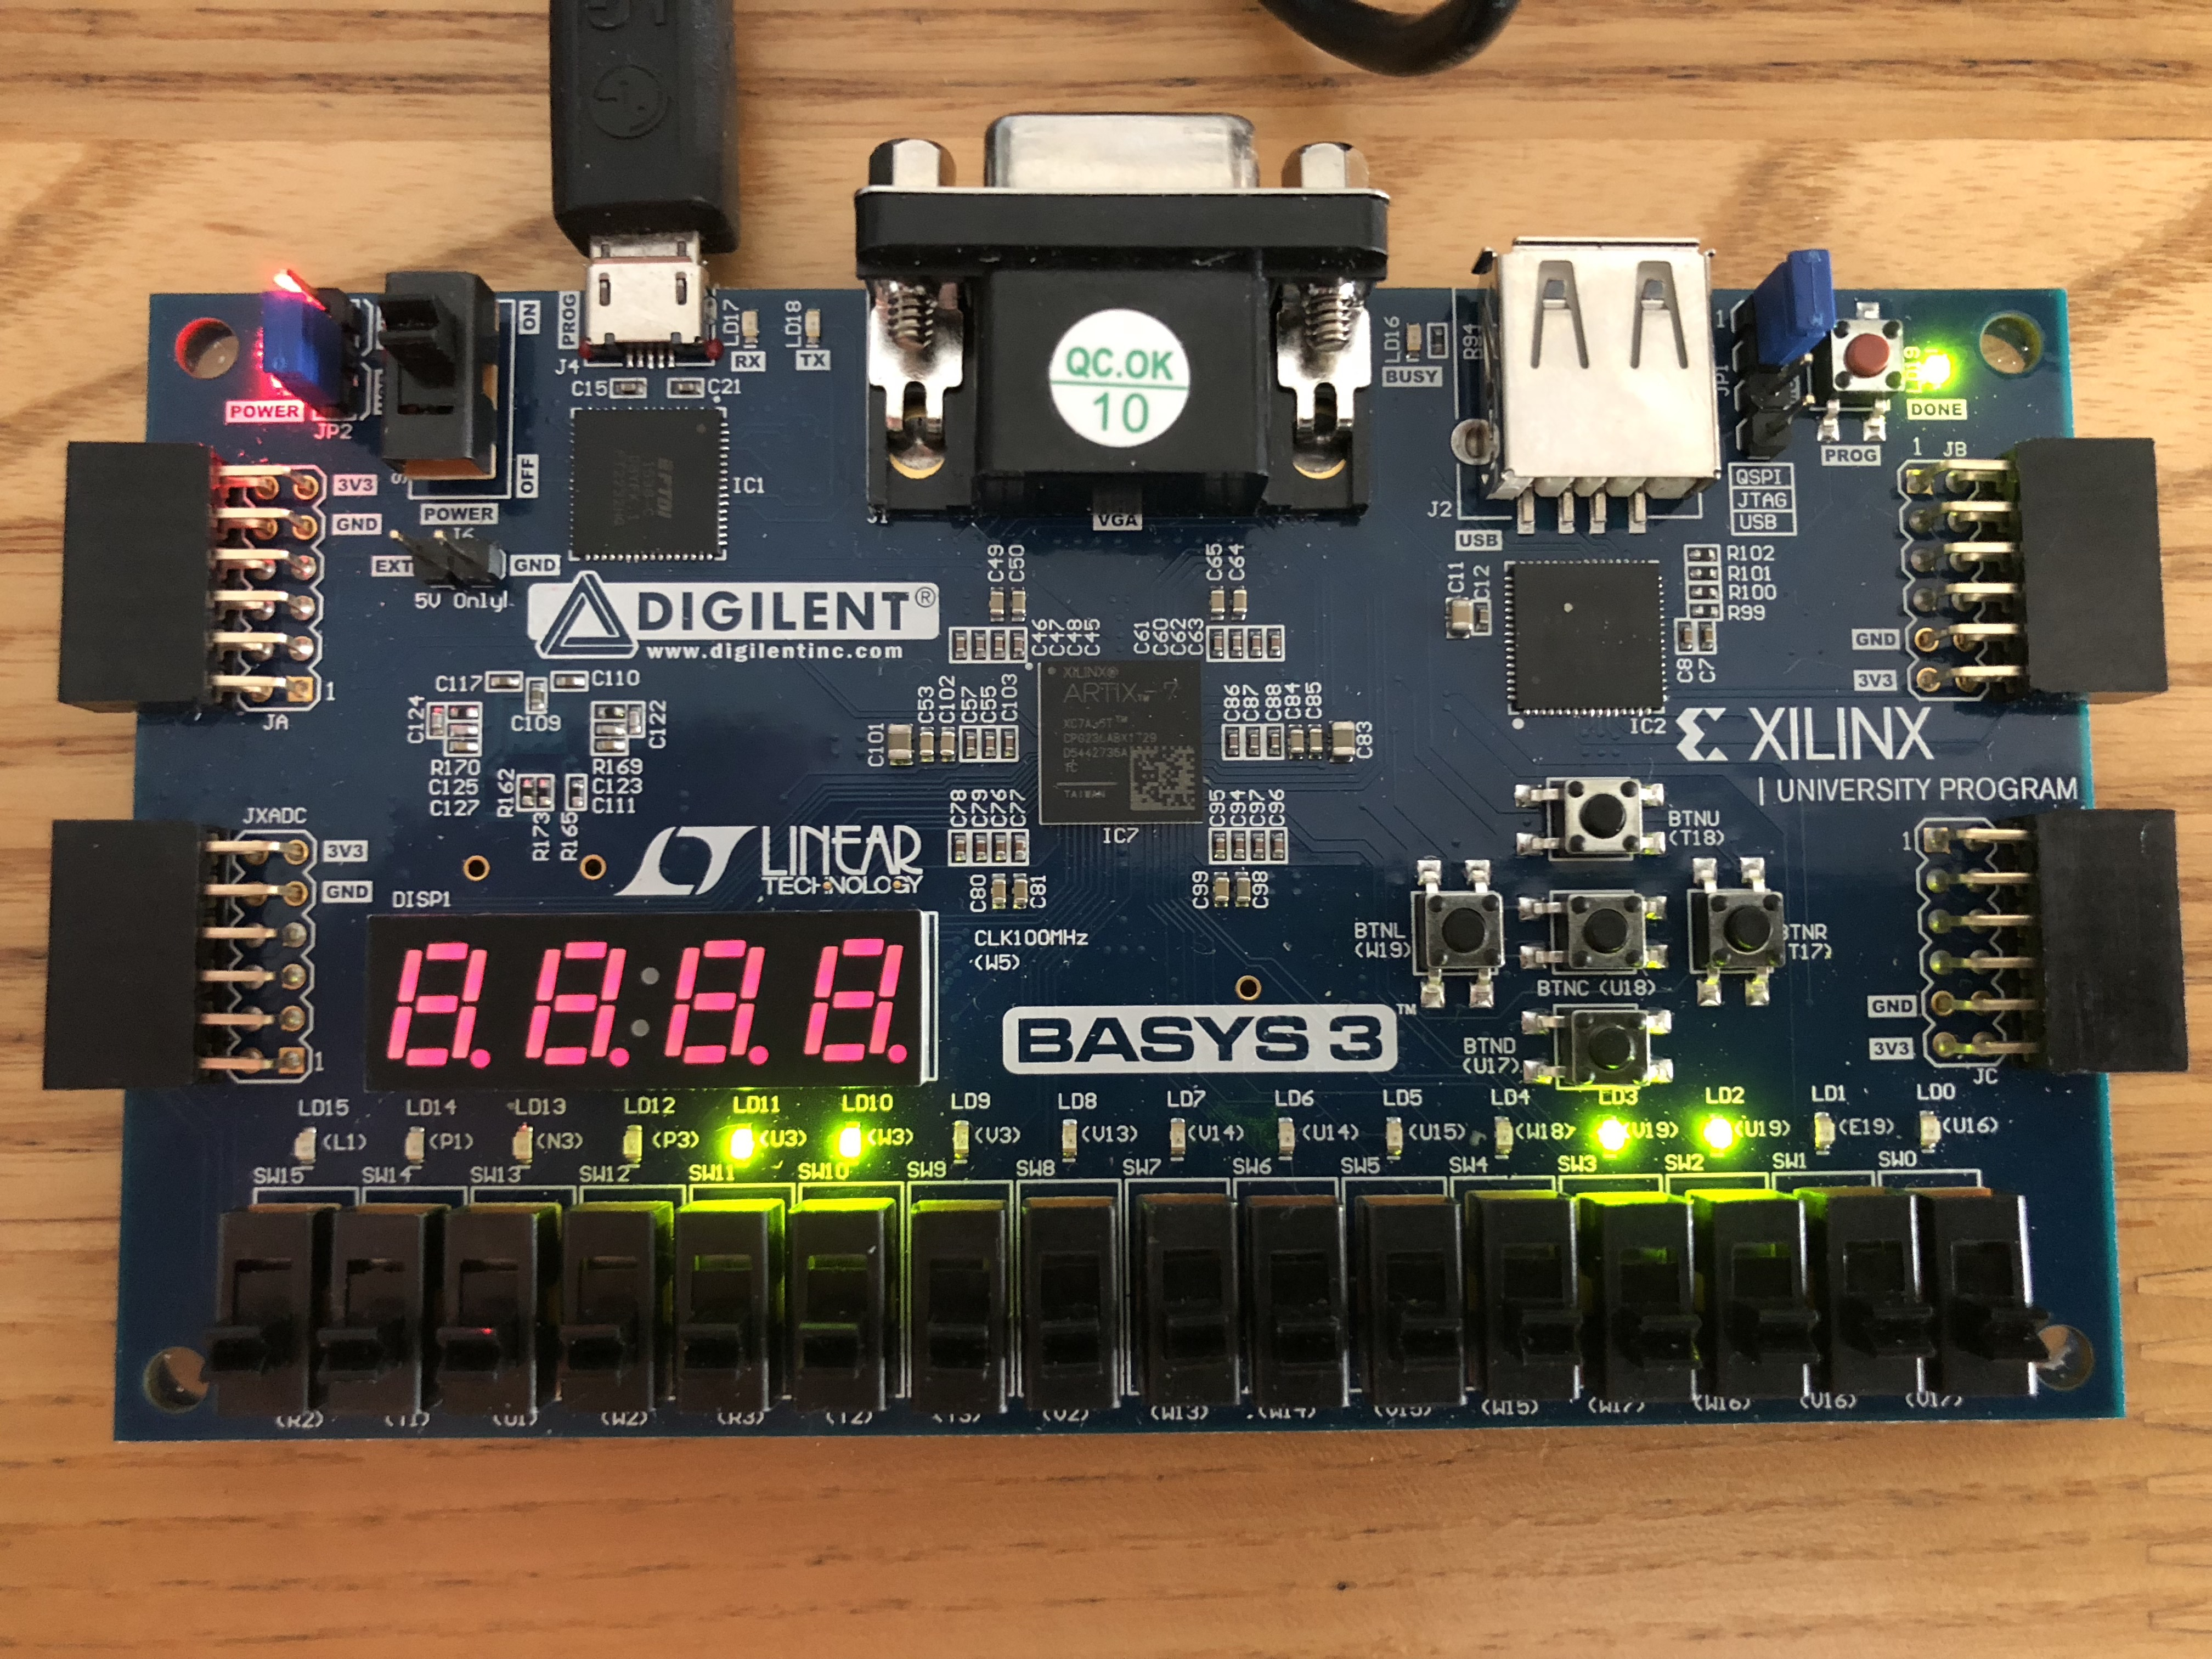
\includegraphics[width=0.5\textwidth]{./images/Part1/l9p1img1.jpg}
	\caption{\label{fig:part1_img1}Standard state, North and South are green, East/West is red.}
\end{center}
\end{figure}

\section{Conclusion}
%Conclude some shit

\pagebreak

\textbf{Appendices}

\begin{appendices}

\section{Clock Divider VHDL Code}
This code for a clock divider is used in the lab.

\begin{lstlisting}[language=VHDL]
library IEEE;
use IEEE.STD_LOGIC_1164.ALL;
use IEEE.NUMERIC_STD.ALL;

entity Clockdivider is
     port(clk : in std_logic;
          start_timer : in std_logic;
	  FastClock,MediumClock,SlowClock, led0 : out std_logic);
end Clockdivider;

architecture clockdivider_arch of Clockdivider is
signal slowClock_sig : STD_LOGIC;
begin
    process  
    variable cnt :	std_logic_vector(26 downto 0):=
     "000000000000000000000000000";
    begin					 
        wait until ((clk'EVENT) AND (clk = '1'));
		if (start_timer = '1') then
	       cnt := "000000000000000000000000000";
	    else  
           cnt := STD_LOGIC_VECTOR(unsigned(cnt) + 1);
	    end if;
   	    FastClock <= cnt(22);
   	    MediumClock <= cnt(24);	
   	    SlowClock <= cnt(26);
        slowClock_sig <= cnt(26);
        if (slowClock_sig = '1') then
		  led0 <= '1';
	    else
		  led0 <= '0';
	    end if;
	end process;
end clockdivider_arch;
\end{lstlisting}

\section{Problem 1 VHDL Code}

\begin{lstlisting}[language=VHDL]
library IEEE;
use IEEE.STD_LOGIC_1164.ALL;

entity vending_machine is
    Port ( clk, reset, nickel, dime, gum, candy : in STD_LOGIC;
    amount : out STD_LOGIC_VECTOR(4 downto 0);
    dispense_gum, dispense_candy, clock_led : out STD_LOGIC);
end vending_machine;

architecture Behavioral of vending_machine is

component clock_divider is
     port(clk : in std_logic;
          start_timer : in std_logic;
	  FastClock,MediumClock,SlowClock, led0 : out std_logic);
end component clock_divider;

signal current_state : STD_LOGIC_VECTOR(2 downto 0) := "000";
signal next_state : STD_LOGIC_VECTOR(2 downto 0) := "000";
signal reset_clock : STD_LOGIC := '0';
signal fast_clock, medium_clock, slow_clock : STD_LOGIC;

begin

    cd : clock_divider port map(clk, reset_clock, fast_clock, 
    		medium_clock, slow_clock, clock_led);

    process(slow_clock, reset)
    begin
        if(reset = '1') then next_state <= "000";
        elsif(slow_clock'event and slow_clock = '1') then
            case current_state is
                when "000" =>
                    if(dime = '1') then next_state <= "010";
                    elsif(nickel = '1') then next_state <= "001";
                    else next_state <= "000";
                    end if;
                when "001" =>
                    if(dime = '1') then next_state <= "011";
                    elsif(nickel = '1') then next_state <= "010";
                    else next_state <= "001";
                    end if;
                when "010" =>
                    if(dime = '1') then next_state <= "100";
                    elsif(nickel = '1') then next_state <= "011";
                    else next_state <= "010";
                    end if;
                when "011" =>
                    if(dime = '1' or nickel = '1') then next_state <= "100";
                    elsif(gum = '1') then next_state <= "101";
                    else next_state <= "011";
                    end if;
                when "100" =>
                    if(candy = '1') then next_state <= "110";
                    elsif(gum = '1') then next_state <= "101";
                    else next_state <= "100";
                    end if;
                when others =>
                    next_state <= "000";
            end case;
        end if;
    end process;
    process(current_state)
    begin
        case current_state is
            when "000" =>
                amount <= "00001";
                dispense_gum <= '0';
                dispense_candy <= '0';
            when "001" =>
                amount <= "00010";
                dispense_gum <= '0';
                dispense_candy <= '0';
            when "010" =>
                amount <= "00100";
                dispense_gum <= '0';
                dispense_candy <= '0';
            when "011" =>
                amount <= "01000";
                dispense_gum <= '0';
                dispense_candy <= '0';
            when "100" =>
                amount <= "10000";
                dispense_gum <= '0';
                dispense_candy <= '0';
            when "101" =>
                amount <= "00001";
                dispense_gum <= '1';
                dispense_candy <= '0';
            when "110" =>
                amount <= "00001";
                dispense_gum <= '0';
                dispense_candy <= '1';
            when others =>
                amount <= "00001";
                dispense_gum <= '0';
                dispense_candy <= '0';
        end case;
    end process;
    current_state <= next_state;

end Behavioral;
\end{lstlisting}

\section{Problem 1 Constraints File}
\begin{center}
\begin{figure}[H]
	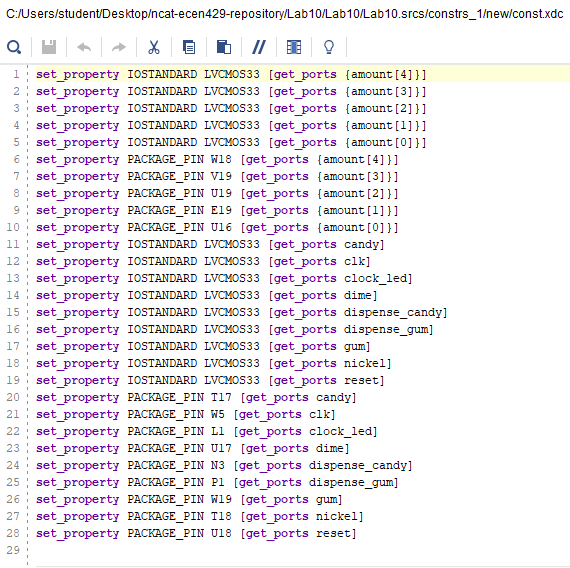
\includegraphics[scale=1]{./images/const.png}
	\caption{\label{fig:Prob1Const}Constraints file for Lab 10.}
\end{figure}
\end{center}

\end{appendices}
\end{document}
